\documentclass{ximera}

\newcommand{\RR}{\mathbb R}
\renewcommand{\d}{\,d}
\newcommand{\dd}[2][]{\frac{d #1}{d #2}}
\renewcommand{\l}{\ell}
\newcommand{\ddx}{\frac{d}{dx}}
\newcommand{\dfn}{\textbf}
\newcommand{\eval}[1]{\bigg[ #1 \bigg]}



\outcome{Use Pythagorean identities to simplify expressions.}
\outcome{Substitute trigonometric functions to simiplify integrals.}
\outcome{Complete the square to change the form of an integral.}
\author{Bart Snapp and Jason Miller}

\title[Dig-In:]{Trigonometric substitution}

\begin{document}
\begin{abstract}
  We integrate by substitution with the appropriate trigonometric
  function.
\end{abstract}
\maketitle

We have seen that the definite integral can be interpreted as giving us the signed area under the curve. Consider the integral 

\[
\int_{-1}^1 \sqrt{1-x^2} \d x
\]

 This integral can be interpreted as area of the following region:
\begin{image}
  \begin{tikzpicture}
    \begin{axis}[
        width=6in,
        %height=3in,
        unit vector ratio*=1 1 1,            
        xmin=-1.1, xmax=1.1,ymin=-.1,ymax=1.1,
        axis lines =center, xlabel=$x$, ylabel=$y$,
        every axis y label/.style={at=(current axis.above origin),anchor=south},
        every axis x label/.style={at=(current axis.right of origin),anchor=west},
        axis on top,
      ] 
      \addplot [draw=none, fill=fillp,samples=200,domain=-1:1] {sqrt(1-x^2)} \closedcycle;
      
      \addplot [penColor,very thick,samples=200,domain=-1:1] {sqrt(1-x^2)};
    \end{axis}
  \end{tikzpicture}
\end{image}

\begin{question}
  Using the graph above and basic facts from geometry, compute:
  \[
  \int_{-1}^1 \sqrt{1-x^2} \d x = \answer{\pi/2}
  \]
\end{question}

We now know a number of integration techniques, yet we are still
unable to evaluate the above integral without resorting to a geometric
interpretation!  This section introduces \dfn{trigonometric substitution},
a method of integration that will give us a new tool in our quest to compute more antiderivatives.
This technique works on the same principle as substitution. Recall the
substitution formula.

\begin{theorem}[Integral Substitution Formula]\index{integral substitution formula} 
If $g$ is differentiable on the interval $[a,b]$ and $f$ is
continuous on the interval $[g(a),g(b)]$, then
\[
\int_a^b f(g(x)) g'(x) \d x =\int_{g(a)}^{g(b)} f(u) \d u.
\]
\end{theorem}

The idea behind substitution is that by changing the variable of integration from $x$ to $u$, then in many cases we can 
simplify the integrand to a form that we can integrate directly. In previous sections, 
we used this result to go from the left integral to the right integral. But what if we tried going from right to left? 


Let's rewrite the substitution formula in a more suggestive manner for our purposes:



\begin{image}
  \begin{tikzpicture}[scale=1,every node/.style={transform shape}]
    \draw [->, line width=10, penColor!10!background] (-1,0)--(.5,0);
    \node at (0,0) {
      $\int_{x(a)}^{x(b)} f(x) \d x=\int_a^b f(x(\theta)) x'(\theta) \d \theta$
    };
  \end{tikzpicture}
\end{image}

This is just the substitution formula again but now we are thinking of transforming from left-to-right.  Initially this may seem to complicate matters. We go from a simple integral to one that looks more complicated. 
However in certain cases we may not know how to integrate $f(x)$, but we may be able to integrate 
$f(x(\theta)) x'(\theta)$. 


We start by applying this technique to compute the area that we previously used
geometry to compute.

\begin{example}
  Compute:
  \[
  \int_{-1}^1 \sqrt{1-x^2} \d x
  \]
  \begin{explanation}\index{Pythagorean identity}

    The difficulty with this integral is that we have a square root of a difference of two terms.
    We can't directly simplify such an expression. (Recall:  $\sqrt{a^2-b^2} \neq \sqrt{a^2} - \sqrt{b^2}$.)  However, consider the Pythagorean identity:
    \[
    \cos^2(\theta) + \sin^2(\theta) = 1
    \]
    From this we see that $\cos^2(\theta)=
    \answer[given]{1-\sin^2(\theta)}$.


   If our expression was $\sqrt{1-\sin^{2}(\theta)}$ then we could simplify.
   We could write 

\[
\sqrt{1-\sin^{2}(\theta)}=\sqrt{\cos^{2}(\theta)}=|\cos(\theta)|
\]
%
%Thus we have taken an expression that involved a square root of a difference of two terms and
%replaced it with a single trigonometric expression that is easier to work with. 

This suggests that it would be useful to use a substitution $x=\sin(\theta)$. 

\begin{remark}
To be more precise, we want to introduce a new variable $\theta=\arcsin(x)$. 
Note that since $\theta$ is the output of the $\arcsin$ function, we must have $\frac{-\pi}{2} \leq \theta \leq \frac{\pi}{2} $, but we will work with the $x=\sin(\theta)$ form during our substitution.
\end{remark}

Just as in the case of substitutions that we have worked with previously, we must convert the entire integral to be in terms of the new variable $\theta$. 
We must also convert  $\d x$ as well as the bounds on the integral.

    \begin{align*}
      x &=\sin(\theta),\\
      \d x &= \cos(\theta) \d\theta,
    \end{align*}

   Now we change our limits of
    integration. We have 

    \begin{align*}
      x &= 1,\\
      \sin(\theta) &= 1,\\
      \theta &= \answer[given]{\pi/2},
    \end{align*}
    and
    \begin{align*}
      x &= -1,\\
      \sin(\theta) &= -1,\\
      \theta &= \answer[given]{-\pi/2}.
    \end{align*}
    Now we may transform our integral via
    \begin{image}
      \begin{tikzpicture}[scale=1,every node/.style={transform shape}]
        \draw [->, line width=10, penColor!10!background] (-1,0)--(.5,0);
        \node at (0,0) {
          $\int_{x(a)}^{x(b)} f(x) \d x=\int_a^b f(x(\theta)) x'(\theta) \d \theta$
        };
      \end{tikzpicture}
    \end{image}
    \begin{align*}
      \int_{-1}^1\sqrt{1-x^2} \d x &= \int_{\answer[given]{-\pi/2}}^{\answer[given]{\pi/2}} \sqrt{1-\sin^2(\theta)} \cdot \cos(\theta) \d \theta \\
      &= \int_{\answer[given]{-\pi/2}}^{\answer[given]{\pi/2}} \sqrt{\cos^2(\theta)}\cdot \cos(\theta) \d\theta \\
      &=\int_{\answer[given]{-\pi/2}}^{\answer[given]{\pi/2}} |\cos(\theta)| \cos\theta \d\theta.
    \end{align*}
    
Now we must do something about the absolute value. Remember that since we 
introduced $\theta=\arcsin(\theta)$, this means $\theta$ lies in $[- \pi/2, \pi/2 ]$. 
Since on $[-\pi/2,\pi/2]$, the function $\cos(\theta)$ is always
    \wordChoice{\choice[correct]{positive}\choice{negative}\choice{zero}},
    we can drop the absolute value, and then employ a power-reduction
    formula\index{power-reduction formula}

    \[
    \cos^2(\theta)= \frac{1+\cos(2\theta)}{2}.
    \]

    Now we have

    \begin{align*}
      &= \int_{-\pi/2}^{\pi/2} \cos^2(\theta) \d \theta \\
      &= \int_{-\pi/2}^{\pi/2} \frac{1+\cos(2\theta)}{2} \d \theta\\
      &= \frac{1}{2} \eval{\answer[given]{\theta +\frac{1}{2}\sin(2\theta)}}_{-\pi/2}^{\pi/2}\\
      &=\answer[given]{\frac{\pi}{2}}.
    \end{align*}

    This matches the answer that we obtained previously using geometry. 


As you may recall, there are two ways to use substitution. Above we
transformed the limits of integration, and worked with the variable
$\theta$. However, we could have solved the problem by finishing with
an antiderivative in $x$ and then evaluating from the original $x$-bounds $-1$ to $1$. We should
familiarize ourselves with this method as well since it will be our only option if we need to do 
an indefinite integral using trig substitution. 

 Above we found the antiderivative 
\[
\int \sqrt{1-x^{2}} \d x=\int \cos^{2}(\theta) \d \theta=\frac{\theta}{2} +\frac{1}{4}\sin(2\theta) + C
\]

    However, now we must express our answer in terms of $x$. Now since $x=\sin(\theta)$, we know
that $\theta=\arcsin(x)$. However what about the $\sin(2\theta)$ term? 
You may be tempted to just stick $\theta=\arcsin(x)$ in this term but we can do better and express the antiderivative
in a simpler form. 
   
    To convert our answer to a function in $x$, we construct a right triangle. 

  Recall that 

\[
\sin(\theta)=\frac{ Opposite}{Hypotenuse}
\]

 Since our substitution was 
$\sin(\theta)=\frac{x}{1}$, we can think of $x$ as the length of the side opposite the angle $\theta$ 
and we can think of $1$ as the length of the hypotenuse of the right triangle. 

    \begin{image}
      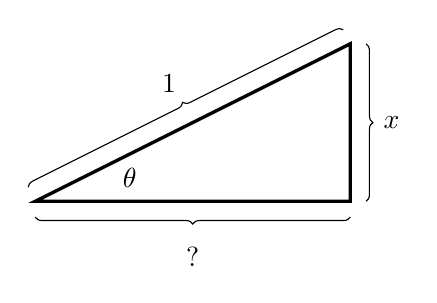
\begin{tikzpicture}
        \coordinate (C) at (0,2);
        \coordinate (D) at (4,2);
        \coordinate (E) at (4,4);
        \tkzMarkRightAngle(C,D,E)
        \tkzMarkAngle(D,C,E)
        \draw[decoration={brace,mirror,raise=.2cm},decorate,thin] (0,2)--(4,2);
        \draw[decoration={brace,mirror,raise=.2cm},decorate,thin] (4,2)--(4,4);
        \draw[decoration={brace,raise=.2cm},decorate,thin] (0,2)--(4,4);
        \draw[very thick] (D)--(E)--(C)--cycle;
        \node at (2,2-.7) {$?$}; %% adj
        \node[anchor=west] at (4+.3,3) {$x$}; %% opp
        \node at (2-.3,3+.5) {$1$}; %% hyp
        \node at (1.2,2.3) {$\theta$};
      \end{tikzpicture}
    \end{image}
   
We can then use the Pythagorean Theorem
to find the adjacent leg of the triangle. Using $?^{2}+x^{2}=1^{2}$ and solving for $?$ we obtain 
that the length of the adjacent side is $\sqrt{1-x^{2}}$. 

    \begin{image}
      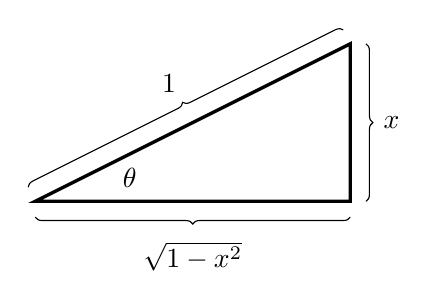
\begin{tikzpicture}
        \coordinate (C) at (0,2);
        \coordinate (D) at (4,2);
        \coordinate (E) at (4,4);
        \tkzMarkRightAngle(C,D,E)
        \tkzMarkAngle(D,C,E)
        \draw[decoration={brace,mirror,raise=.2cm},decorate,thin] (0,2)--(4,2);
        \draw[decoration={brace,mirror,raise=.2cm},decorate,thin] (4,2)--(4,4);
        \draw[decoration={brace,raise=.2cm},decorate,thin] (0,2)--(4,4);
        \draw[very thick] (D)--(E)--(C)--cycle;
        \node at (2,2-.7) {$\sqrt{1-x^{2}}$}; %% adj
        \node[anchor=west] at (4+.3,3) {$x$}; %% opp
        \node at (2-.3,3+.5) {$1$}; %% hyp
        \node at (1.2,2.3) {$\theta$};
      \end{tikzpicture}
    \end{image}

Now we still need to express $\sin(2\theta)$ in terms of $x$ using this triangle. However the angle in our 
right triangle is $\theta$, not $2\theta$. Recall the trig identity

\[
\sin(2\theta)=2\sin(\theta)\cos(\theta)
\]

We can then write our above antiderivative as 
\[
\frac{\theta}{2} +\frac{1}{2}\sin(\theta)\cos(\theta) + C
\]

We can then replace $\sin(\theta)=x$ and using our triangle and the fact that 
\[
\cos(\theta)=\frac{Adjacent}{Hypotenuse}
\]
we can write $\cos(\theta)=\frac{\sqrt{1-x^{2}}}{1}$.

Hence our antiderivative can now be written in terms of $x$:

    \begin{align*}
      \int \sqrt{1-x^2} \d x &= \frac{\theta}{2} +\frac{1}{2}\sin(\theta)\cos(\theta)+C \\
      &= \answer[given]{\frac{\arcsin(x)}{2} + \frac{x\sqrt{1-x^2}}{2}} + C 
    \end{align*}
  \end{explanation}
\end{example}

\begin{question}
  If
  \[
  \int \sqrt{1-x^2} \d x = \frac{\arcsin(x)}{2} + \frac{x\sqrt{1-x^2}}{2} + C,
  \]
  then
  \[
  \int_{-1}^{1}\sqrt{1-x^2} \d x = \answer{\pi/2}
  \]
\end{question}



The key idea with this example was that the expression $\sqrt{1-x^{2}}$ was difficult to work with directly and 
using the substitution $x=\sin(\theta)$ allowed us to simplify the expression and turn the integral 
into a trig integral that was easier to calculate. 


There are other situations where this kind of strategy is useful. Let's look at a few more examples.

\begin{example}
  Compute:
  \[
  \int \frac{x^3}{x^2+9} \d x
  \]
  \begin{explanation}
Here we don't have a square root to contend with but we do have a sum of two 
terms in the denominator. (Recall: It is never ok to split a fraction over a sum or difference in the denominator!)   It would be nice if there was some way to simplify the denominator into just one term. 

   Recall one of the alternate forms of the Pythagorean identity
    \[
    \tan^2(\theta) + 1 = \answer[given]{\sec^2(\theta)}
    \]
    and note that multiplying the entire equation by $9$ yields
    \[
    \left(\answer[given]{3\tan(\theta)}\right)^2 + 9 = (3\sec(\theta))^2
    \]

This suggests that if we made the substitution $x=3\tan(\theta)$ then we could
use this trig identity to simplify the denominator of our integrand. 

    Hence we'll make the substitution
    \begin{align*}
      x &= 3\tan(\theta),\\
      \d x &= \answer[given]{3\sec^2(\theta)} \d \theta,
    \end{align*}

\begin{remark}
More precisely, this means that we are introducting a new variable $\theta=\arctan\left(\frac{x}{3}\right)$ 
and then rewriting it as $x=3\arctan(\theta)$ since that is a more useful form 
for our given problem. Since $\theta$ is the output of the $\arctan$ function, we must have
$-\pi/2 < \theta < \pi/2$. 
\end{remark}

Now we convert our integral to be in terms of the new variable $\theta$:

    \begin{align*}
      \int \frac{x^3}{x^2+9} \d x &= \int \frac{(3\tan(\theta))^3}{(3\tan(\theta))^2+9} \cdot 3\sec^2(\theta) \d \theta\\
      &=\int \frac{(3\tan(\theta))^3}{(3\sec(\theta))^2} \cdot 3\sec^2(\theta) \d \theta\\
      &=9\int \tan^3(\theta)  \d \theta.
    \end{align*}
    We'll use our expertise with trigonometric integrals
    \begin{align*}
      9\int \tan^3(\theta)  \d \theta &= 9\int \frac{\sin^3(\theta)}{\cos^{3}(\theta)}  \d \theta\\
      &= 9\int \frac{\sin^2(\theta) \sin(\theta)}{\cos^{3}(\theta)}  \d \theta\\
      &= 9\int \frac{(1-\cos^2(\theta)) \sin(\theta)}{\cos^{3}(\theta)}   \d \theta
    \end{align*}
    Now we do another substitution
    \begin{align*}
      u&=\cos(\theta),\\
      \d u &= \answer[given]{-\sin(\theta)}\d \theta,
    \end{align*}
    to find
    \begin{align*}
      &= -9\int \frac{1-u^2}{u^3}\d u\\
      &= -9\int u^{-3}-\frac{1}{u}\d u\\
      &= -9\left(\answer[given]{\frac{u^{-2}}{-2}}-\ln|u|\right) + C\\
      &= \frac{9}{2u^2} + 9\ln|u| + C.
    \end{align*}

. Since $u = \cos(\theta)$ we have

    \[
    \frac{9}{2u^2} + 9\ln|u| + C = \frac{9}{2\cos^2(\theta)} + 9\ln|\cos(\theta)| + C.
    \]

    Now that we have an answer in terms of $\theta$, we must convert it back to
    being a function in $x$.
    To convert our answer to a function in $x$, use a reference right
    triangle, noting that $3\tan(\theta) = x$, and so $\tan(\theta) =
    x/3$. 
Since 
\[
\tan(\theta)=\frac{Opposite}{Adjacent}
\] 
we can label the triangle with $x$ as the length of the opposite side and $3$ as the length of the adjacent side. Note we have already used the Pythagorean Theorem to 
find the length of the hypotenuse. 

    \begin{image}
      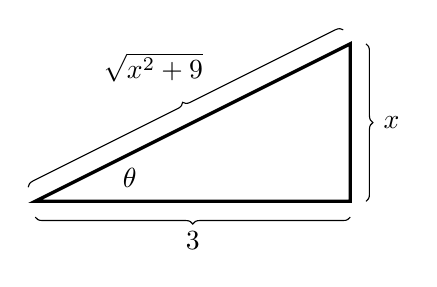
\begin{tikzpicture}
        \coordinate (C) at (0,2);
        \coordinate (D) at (4,2);
        \coordinate (E) at (4,4);
        \tkzMarkRightAngle(C,D,E)
        \tkzMarkAngle(D,C,E)
        \draw[decoration={brace,mirror,raise=.2cm},decorate,thin] (0,2)--(4,2);
        \draw[decoration={brace,mirror,raise=.2cm},decorate,thin] (4,2)--(4,4);
        \draw[decoration={brace,raise=.2cm},decorate,thin] (0,2)--(4,4);
        \draw[very thick] (D)--(E)--(C)--cycle;
        \node at (2,2-.5) {$3$}; %% adj
        \node[anchor=west] at (4+.3,3) {$x$}; %% opp
        \node at (2-.5,3+.7) {$\sqrt{x^{2}+9}$}; %% hyp
        \node at (1.2,2.3) {$\theta$};
      \end{tikzpicture}
    \end{image}
    Thus
    \[
    \cos(\theta) =  \answer[given]{\frac{3}{\sqrt{x^{2}+9}}}
    \]

    and we may write

    \begin{align*}
      \int \frac{x^3}{x^2+9} \d x &= \frac{9}{2\cos^2(\theta)} + 9\ln|\cos(\theta)| + C\\
      &= \frac{x^{2}+9}{2} + 9 \ln\left(\frac{3}{\sqrt{x^{2}+9}}\right) + C.
    \end{align*}


  \end{explanation}
\end{example}


\begin{example}
Compute 

\[
\int_{4\sqrt{2}}^{8} \frac{1}{ x^{2}\sqrt{x^{2}-16}} \d x \text{ where } x > 4
\]

\begin{explanation}
Again we have a square root of a difference of two terms. However unlike the $\sqrt{1-x^{2}}$ we encountered 
in the first example of this section, a substitution involving $\sin(\theta)$ will not allow us to simplify 
the square root. Instead we rewrite the form of the Pythagorean identity used in the previous example to get 

\[
\sec^{2}(\theta)-1=\tan^{2}(\theta)
\]

This suggests that we should use 

 \begin{align*}
      x &= 4\sec(\theta),\\
      \d x &= \answer[given]{4\sec(\theta)\tan(\theta)} \d \theta,
    \end{align*}

\begin{remark}
This means we are introducting a new variable $\theta=\arcsec\left(\frac{x}{4}\right)$. 
In this problem, since $x > 4$, we must have $0 \leq \theta < \pi/2 $.  In general, one must be careful about which branch of $\arcsec$ needs to be used. 
\end{remark}
Let's also go ahead and change our limits of integration:


    \begin{align*}
      x &= 4\sqrt{2},\\
     4 \sec(\theta) &=4\sqrt{2},\\
       \cos(\theta)&=\frac{1}{\sqrt{2}}, \\
      \theta &= \answer[given]{\frac{\pi}{4}},
    \end{align*}
    and
    \begin{align*}
      x &= 8,\\
     4 \sec(\theta) &= 8,\\
        \cos(\theta)&=\frac{1}{2}, \\
      \theta &= \answer[given]{\frac{\pi}{3}}.
    \end{align*}


Now we convert our integral to be in terms of the new variable $\theta$:

    \begin{align*}
      \int_{4\sqrt{2}}^{8} \frac{1}{x^{2}\sqrt{x^{2}-16}} \d x &= \int_{\frac{\pi}{4}}^{\frac{\pi}{3}} \frac{ 4\sec(\theta)\tan(\theta)}{ 4^{2}\sec^{2}(\theta) \sqrt{ 16(\sec^{2}(\theta)-1) }} \d \theta \\
      &=\frac{1}{16}\int_{\frac{\pi}{4}}^{\frac{\pi}{3}} \frac{\tan(\theta)}{\sec(\theta) |\tan(\theta)|}  \d \theta
          \end{align*}

The fact that $0\leq \theta < \pi/2$ guarantees that $\tan(\theta) \geq 0$. 
 
   Now we can evaluate the integral:
    \begin{align*}
     \frac{1}{16}\int_{\frac{\pi}{4}}^{\frac{\pi}{3}} \frac{\tan(\theta)}{\sec(\theta) \tan(\theta)}  \d \theta &= \frac{1}{16} \int_{\frac{\pi}{4}}^{\frac{\pi}{3}} \answer[given]{\cos(\theta)}  \d \theta\\
      &= \eval{\frac{1}{16}\answer[given]{\sin(\theta)}}_{\frac{\pi}{4}}^{\frac{\pi}{3}}= \answer[given]{\frac{\sqrt{3}-\sqrt{2}}{32}}
         \end{align*}




\end{explanation}
\end{example}



























%\begin{example}
%Compute 
%
%\[
%\int_{4}^{8} x^{3}\sqrt{x^{2}-16} \d x \text{ where } x \geq 4
%\]
%
%\begin{explanation}
%Again we have a square root of a difference of two terms. However unlike the $\sqrt{1-x^{2}}$ we encountered 
%in the first example of this section, a substitution involving $\sin(\theta)$ will not allow us to simplify 
%the square root. Instead we rewrite the form of the Pythagorean identity used in the previous example to get 
%
%\[
%\sec^{2}(\theta)-1=\tan^{2}(\theta)
%\]
%
%This suggests that we should use 
%
% \begin{align*}
%      x &= 4\sec(\theta),\\
%      \d x &= \answer[given]{4\sec(\theta)\tan(\theta)} \d \theta,
%    \end{align*}
%
%\begin{remark}
%This means we are introducting a new variable $\theta=\arcsec\left(\frac{x}{4}\right)$. 
%In this problem, since $x \geq 4$, we must have $0 \leq \theta < \pi/2 $.  In general, one must be careful about which branch of $\arcsec$ needs to be used. 
%\end{remark}
%Let's also go ahead and change our limits of integration:
%
%
%    \begin{align*}
%      x &= 4,\\
%     4 \sec(\theta) &=4,\\
%       \cos(\theta)&=1, \\
%      \theta &= \answer[given]{0},
%    \end{align*}
%    and
%    \begin{align*}
%      x &= 8,\\
%     4 \sec(\theta) &= 8,\\
%        \cos(\theta)&=\frac{1}{2}, \\
%      \theta &= \answer[given]{\frac{\pi}{3}}.
%    \end{align*}
%
%
%Now we convert our indefinite integral to be in terms of the new variable $\theta$:
%
%    \begin{align*}
%      \int_{4}^{8} x^{3}\sqrt{x^{2}-16} \d x &= \int_{0}^{\frac{\pi}{3}} 4^{3}\sec^{3}(\theta) \sqrt{16(\sec^{2}(\theta)-1)}\cdot 4\sec(\theta)\tan(\theta) \d \theta \\
%      &=\int_{0}^{\frac{\pi}{3}} 4^{5} \sec^{4}(\theta) |\tan(\theta)| \tan(\theta) \d \theta
%          \end{align*}
%
%The fact that $0\leq \theta < \pi/2$ guarantees that $\tan(\theta) \geq 0$. 
% 
%   Now we can evaluate the indefinite trig integral:
%    \begin{align*}
%      4^{5}\int \sec^{4}(\theta)\tan^2(\theta)  \d \theta &= 4^{5}\int \sec^{2}(\theta)\tan^{2}(\theta) \sec^{2}(\theta)  \d \theta\\
%      &= 4^{5} \int  (\tan^{2}(\theta) + 1) \tan^{2}(\theta) \sec^{2}(\theta) \d \theta
%         \end{align*}
%
%    Now we do another substitution
%    \begin{align*}
%      u&=\tan(\theta),\\
%      \d u &= \answer[given]{ \sec^{2}(\theta)}\d \theta,
%    \end{align*}
%    to find
%    \begin{align*}
%      &= 4^{5}\int ( u^{2}+1) u^{2} \d u\\
%      &= 4^{5}\int u^{4}+u^{2}\d u\\
%      &= 4^{5}\left(\answer[given]{\frac{u^{5}}{5}}+\frac{u^{3}}{3} \right) + C\\
%      &=4^{5} \left( \frac{\tan^{5}(\theta)}{5} + \frac{\tan^{3}(\theta)}{3} \right) + C
%    \end{align*}
%
%Now we go back to the definite integral 
%
%
%\begin{align*}
%\int_{4}^{8} x^{3}\sqrt{x^{2}-16} \d x&=4^{5}\int_{0}^{\frac{\pi}{3}} \sec^{4}(\theta)\tan^{2}(\theta) \d \theta \\
% &=\eval{4^{5} \left( \frac{\tan^{5}(\theta)}{5} + \frac{\tan^{3}(\theta)}{3} \right)}_{0}^{\frac{\pi}{3}} \\
%                       &=\answer[given]{   \frac{4^{5}14\sqrt{3}}{5}  }                                                                                       
%\end{align*}
%
%
%
%\end{explanation}
%\end{example}

So far we have seen that we can use trig substitutions to simplify expressions
like $x^{2}-a^{2}$, $a^{2}-x^{2}$, and $x^{2}+a^{2}$. 
However, sometimes the integral may not be in a form where it is clear that a trig substitution 
will help. 
One very useful tool is to \dfn{complete the square}, and then choose a
trigonometric function which allows the use of a Pythagorean identity
to simplify the expression. 

Let's recall how to complete the square for a general quadratic $ax^2+bx+c$.  First we divide through by $a$.
\begin{align*}
x^{2}+\frac{b}{a}x+\frac{c}{a} &=x^{2}+\frac{b}{a}+\left(\frac{b}{2a}\right)^{2}-\left(\frac{b}{2a}\right)^{2}+\frac{c}{a} \\
&=\left(x+\frac{b}{2a}\right)^{2}+\left(\frac{c}{a}-\left(\frac{b}{2a}\right)^{2}\right)
\end{align*}

Now, consider the following example:


\begin{example}
  Compute:
  \[
  \int \frac{\sqrt{x^2+6x+5}}{x+3}\d x \text{ where } x \geq -1
  \]

  \begin{explanation}
  Initially it does not seem that a trig sub would help, but let's complete the square on the quadratic under the square root.

    \begin{align*}
      x^2+6x+5 &= x^2+6x+\answer[given]{9}+(5-\answer[given]{9})\\
      &= (\answer[given]{x+3})^2-4
    \end{align*}
    Our integral becomes

    \[
    \int \frac{\sqrt{(x+3)^2-4}}{x+3}\d x
    \]

    We want to let $(x+3)$ equal some trigonometric
    function that will simplify after the application of a
    Pythagorean identity. Again 

    \[
    \tan^2(\theta) + 1 = \sec^2(\theta)
    \]
    will be helpful. We multiple this equation by $4$ and rearrange to find
    \[
    (\answer[given]{2\tan(\theta)})^2 = (\answer[given]{2\sec(\theta)})^2 - 4
    \]

    Thus we use the substitution 
    \begin{align*}
      (x+3) &=  2\sec(\theta)\\
      \d x &= 2\sec(\theta)\tan(\theta) \d \theta.
    \end{align*}
    So making this substitution we have
    \begin{align*}
      \int &\frac{\sqrt{(x+3)^2-4}}{x+3}\d x \\
      &= \int\frac{\sqrt{(\answer[given]{2\sec(\theta)})^2-4}}{\answer[given]{2\sec(\theta)}} \cdot 2\sec(\theta)\tan(\theta)\d \theta\\
      &= \int\frac{\sqrt{4\tan^{2}(\theta)}}{2\sec(\theta)} \cdot 2\sec(\theta)\tan(\theta)\d \theta\\
    \end{align*}
    Since $x\geq -1$, this guarantees that $0\leq \theta \leq \pi/2$ and thus that 
$\tan(\theta) \geq 0$:

    \[
    \int 2 \tan^2(\theta) \d \theta = 2\int \tan^2(\theta) \d \theta
    \]

    We'll again use the Pythagorean identity
    \[
    \tan^2(\theta) + 1 = \sec^2(\theta)
    \]
    to write
    \begin{align*}
      &= 2\int \sec^2(\theta) - 1 \d \theta\\
      &= \answer[given]{2\left(\tan(\theta) - \theta\right)} + C
    \end{align*}
    Now that we have an answer in $\theta$, we must convert it back to
    being a function in $x$. Since $x+3 = 2\sec(\theta)$ we have
    \[
    \cos(\theta) = \frac{2}{x+3},
    \]
    and using a reference triangle and using the Pythagorean Theorem
to find the length of the opposite side we have:
    \begin{image}
      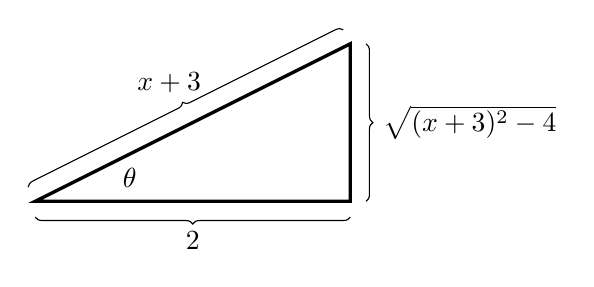
\begin{tikzpicture}
        \coordinate (C) at (0,2);
        \coordinate (D) at (4,2);
        \coordinate (E) at (4,4);
        \tkzMarkRightAngle(C,D,E)
        \tkzMarkAngle(D,C,E)
        \draw[decoration={brace,mirror,raise=.2cm},decorate,thin] (0,2)--(4,2);
        \draw[decoration={brace,mirror,raise=.2cm},decorate,thin] (4,2)--(4,4);
        \draw[decoration={brace,raise=.2cm},decorate,thin] (0,2)--(4,4);
        \draw[very thick] (D)--(E)--(C)--cycle;
        \node at (2,2-.5) {$2$}; %% adj
        \node[anchor=west] at (4+.3,3) {$\sqrt{(x+3)^{2}-4}$}; %% opp
        \node at (2-.3,3+.5) {$x+3$}; %% hyp
        \node at (1.2,2.3) {$\theta$};
      \end{tikzpicture}
    \end{image}
    Thus
    \[
    \tan(\theta) = \answer[given]{\frac{\sqrt{(x+3)^{2}-4}}{2}}
    \]
    and we may write
    \begin{align*}
    \int &\frac{\sqrt{(x+3)^2-4}}{x+3} \d x = 2\left(\tan(\theta) - \theta\right) + C\\
      &= \sqrt{(x+3)^{2}-4} - 2\arctan\left(\frac{\sqrt{(x+3)^{2}-4}}{2}\right) + C.
    \end{align*}
  \end{explanation}
\end{example}

Thus using the technique of completing the square, we can always rewrite any quadratic in a form where a trig
substitution can be used to simplify the expression. 



\section{Summary}

In general, when doing a trig substitution:
\begin{itemize}
\item If the quadratic has the form $a^2 + x^2$ after completing the square, make the substitution $u = a\tan(\theta)$. 
\item If the quadratic has the form $a^2 - x^2$ after completing the square, make the substitution $u = a\sin(\theta)$ 
\item If the quadratic has the form $x^2 - a^2$ after completing the
  square, make the substitution $u = a\sec(\theta)$
\end{itemize}
%Although the choices $a\cot(\theta)$, $a\cos(\theta)$, and $a \csc(\theta)$
%could be used with equal efficiency, the convention is to only use the trig substitutions that we have covered in 
%this section. 

%\begin{remark}
You should always remember the other integration techniques you have learned previously; they may allow you to compute the integral more easily than trig substitutions in some cases. In particular, go back and look at example 2 in this section and see if you can compute this integral using a more efficient integration technique!  In some cases, though, trig substitution will be your only option.
%\end{remark}

\end{document}
